\chapter{Objectives and Criteria}
\section{Detailed Task Description}
The goal of the thesis is to add value to real business documents by aggregating expenses into clusters of similar expenses. The supplied document dataset consists of 150.000 invoices. The invoices contain different information, for example the vendor, billing amount or a description of the goods. Valuable information for companies would be insight into the different categories of expenses and the corresponding cost. With traditional data analysis methods, the company’s controlling departments cannot identify which expenses are similar in nature (for example logistics costs). 

The task is to perform a full data analysis on the supplied dataset. The dataset is to be prepared for processing with established methods. An evaluation for different means of feature extraction, machine learning, model evaluation and visualization should be performed. With the evaluation a complete flow for the data processing should be presented. The result should be an added value to the dataset in the form of aggregated expenses.

\section{Criteria set by SAP SE}
The analysis should be performed utilizing only available resources, which are the student’s company laptop and already available instances for SAP internal services.

\section{Research Model}

To solve the task described in chapter 1.2, this paper employs the \ac{CRISP-DM} \cite{CRISPDM2000}. This model puts forward a structure for conducting data mining projects. \ac{CRISP-DM} was developed in 1996 by three companies, which are now the partners of the \ac{CRISP-DM} consortium: NCR, DaimlerChrysler AG and SPSS Inc. 

A poll \cite{CRISPDMPopular2020} conducted amongst users of a wegpage about data science project management, found that almost half of all respondents most commonly employ the \ac{CRISP-DM} process model. Followed by Scrum and Kanban with a 18\% and 12\% of the user share, \ac{CRISP-DM} is by far the most popular. Other methods such as \ac{KDD} and \ac{SEMMA} are also noteworthy alternatives, but are less popular that CRISP-DM, Scrum and Kanban.

\begin{figure}[ht]
	\centering
	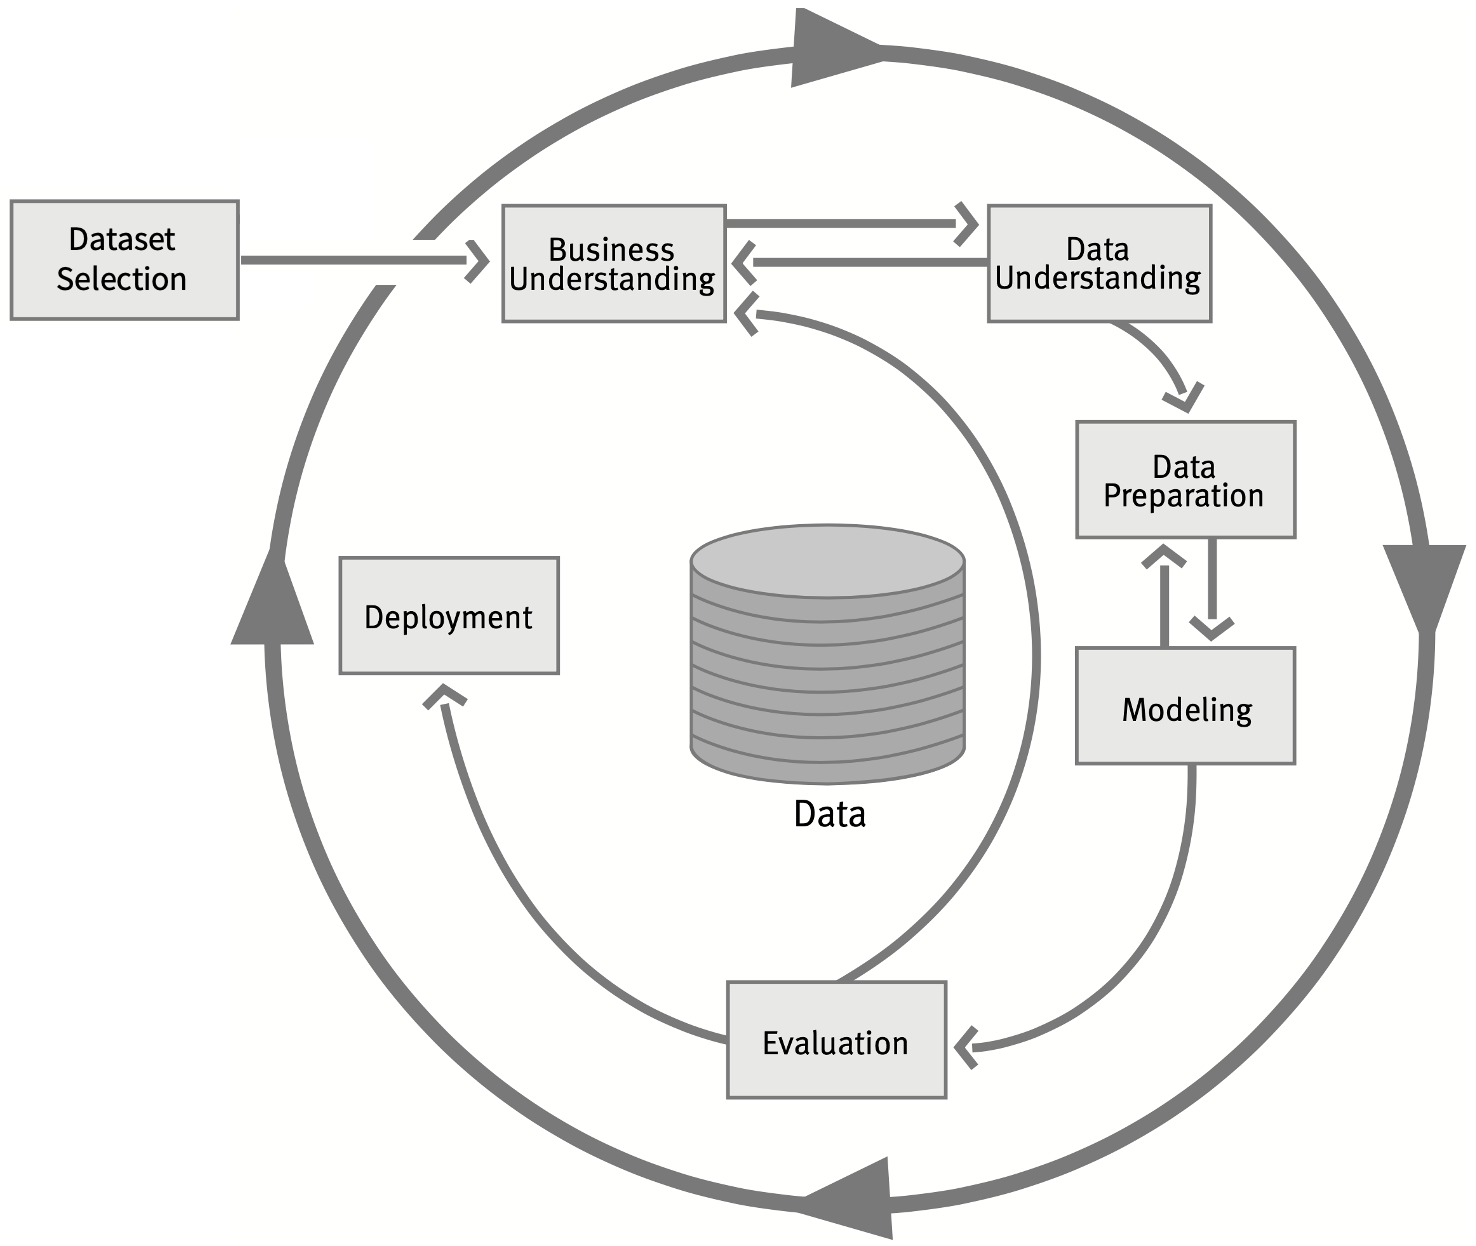
\includegraphics[height=10cm]{Bilder/Research_Model.png}
	\caption{Adjusted CRISP-DM Model}
	\label{fig:CRISM-DM}
\end{figure}

Being the most popular model, \ac{CRISP-DM} not necessarily is the best fit for all data science projects. In the case of this particular research effort, \ac{CRISP-DM} proved the best suit for several reasons.
Firstly, the process model follows the natural intuition of project design for data science tasks. Evaluation has to occur before the deployment, the modelling needs to occur before the evaluation, the preparation needs to occur before the modelling, and an adequate understanding of business and data aspects has to be developed in the beginning of the process. All those elemental dependencies are reflected in the model.
Secondly, the \ac{CRISP-DM} model adresses the iterative nature of data mining. Fundamentally, the model is of circular nature, reflecting the fact that data science projects underly the premise of continuous improvement. After the deployment of one solution, monitoring can give insights which allow for deeper business understanding, triggering the start of a new circuit of the model. Another model which puts forward an iterative approach is \ac{KDD} \cite{KDD}.
Thirdly, the model allows for a tailored trail through its phases: Business Understanding, Data Understanding, Data Preparation, Modeling, Evaluation, and Deployment. The free choice of path is more favorable compared to \ac{KDD}, which allows for loops, but has a fixed order \cite{KDD}.
Fourth, \ac{CRISP-DM} has no special requirements regarding team size or roles. Instead, a \ac{CRISP-DM} project can be completed by only one person. This stands in contrast to SCRUM, which needs different roles represented by people in the team to work effectively \cite{SCRUMSolo}. 
Fifth, the \ac{CRISP-DM} model was publicized in the context of a 70-page guide with generic task descriptions and outputs for each phase \cite{CRISPDM2000}. The detailed guide is especially valuable for teams with little experience, as it prevents tasks being forgotten.

Classically, the reference model consists of six phases. For this thesis the model was adapted to reflect all tasks encompassed. The phase "Dataset Selection" was added, resulting in a total of seven phases. The newly added phase includes the selection of a suitable dataset, the data retrieval, and the data provisioning.

 